\documentclass{tufte-book}

\usepackage{ulem}
\usepackage{amsmath}
\usepackage{amsthm}
\usepackage{amsfonts}
\usepackage{amssymb}

\hypersetup{colorlinks}% uncomment this line if you prefer colored hyperlinks (e.g., for onscreen viewing)

%%
% Book metadata
\title{Problem Sets Vol. II}
\author[Alex Cooper]{Alex Cooper}
\publisher{adrcooper.com}

%%
% If they're installed, use Bergamo and Chantilly from www.fontsite.com.
% They're clones of Bembo and Gill Sans, respectively.
\IfFileExists{bergamo.sty}{\usepackage[osf]{bergamo}}{}% Bembo
\IfFileExists{chantill.sty}{\usepackage{chantill}}{}% Gill Sans

\usepackage{microtype}

%%
% For nicely typeset tabular material
\usepackage{booktabs}

%%
% For graphics / images
\usepackage{graphicx}
\setkeys{Gin}{width=\linewidth,totalheight=\textheight,keepaspectratio}
\graphicspath{{graphics/}}

\usepackage{array}
\providecommand{\tabularnewline}{\\}

% The fancyvrb package lets us customize the formatting of verbatim
% environments.  We use a slightly smaller font.
\usepackage{fancyvrb}
\fvset{fontsize=\normalsize}

%%
% Prints argument within hanging parentheses (i.e., parentheses that take
% up no horizontal space).  Useful in tabular environments.
\newcommand{\hangp}[1]{\makebox[0pt][r]{(}#1\makebox[0pt][l]{)}}

%%
% Prints an asterisk that takes up no horizontal space.
% Useful in tabular environments.
\newcommand{\hangstar}{\makebox[0pt][l]{*}}

%%
% Prints a trailing space in a smart way.
\usepackage{xspace}

%%
% Some shortcuts for Tufte's book titles.  The lowercase commands will
% produce the initials of the book title in italics.  The all-caps commands
% will print out the full title of the book in italics.
\newcommand{\vdqi}{\textit{VDQI}\xspace}
\newcommand{\ei}{\textit{EI}\xspace}
\newcommand{\ve}{\textit{VE}\xspace}
\newcommand{\be}{\textit{BE}\xspace}
\newcommand{\VDQI}{\textit{The Visual Display of Quantitative Information}\xspace}
\newcommand{\EI}{\textit{Envisioning Information}\xspace}
\newcommand{\VE}{\textit{Visual Explanations}\xspace}
\newcommand{\BE}{\textit{Beautiful Evidence}\xspace}

\newcommand{\TL}{Tufte-\LaTeX\xspace}

% Prints the month name (e.g., January) and the year (e.g., 2008)
\newcommand{\monthyear}{%
  \ifcase\month\or January\or February\or March\or April\or May\or June\or
  July\or August\or September\or October\or November\or
  December\fi\space\number\year
}


% Prints an epigraph and speaker in sans serif, all-caps type.
\newcommand{\openepigraph}[2]{%
  %\sffamily\fontsize{14}{16}\selectfont
  \begin{fullwidth}
  \sffamily\large
  \begin{doublespace}
  \noindent\allcaps{#1}\\% epigraph
  \noindent\allcaps{#2}% author
  \end{doublespace}
  \end{fullwidth}
}

% Inserts a blank page
\newcommand{\blankpage}{\newpage\hbox{}\thispagestyle{empty}\newpage}

\usepackage{units}

% Typesets the font size, leading, and measure in the form of 10/12x26 pc.
\newcommand{\measure}[3]{#1/#2$\times$\unit[#3]{pc}}

% Macros for typesetting the documentation
\newcommand{\hlred}[1]{\textcolor{Maroon}{#1}}% prints in red
\newcommand{\hangleft}[1]{\makebox[0pt][r]{#1}}
\newcommand{\hairsp}{\hspace{1pt}}% hair space
\newcommand{\hquad}{\hskip0.5em\relax}% half quad space
\newcommand{\TODO}{\textcolor{red}{\bf TODO!}\xspace}
\newcommand{\ie}{\textit{i.\hairsp{}e.}\xspace}
\newcommand{\eg}{\textit{e.\hairsp{}g.}\xspace}
\newcommand{\na}{\quad--}% used in tables for N/A cells
\providecommand{\XeLaTeX}{X\lower.5ex\hbox{\kern-0.15em\reflectbox{E}}\kern-0.1em\LaTeX}
\newcommand{\tXeLaTeX}{\XeLaTeX\index{XeLaTeX@\protect\XeLaTeX}}
% \index{\texttt{\textbackslash xyz}@\hangleft{\texttt{\textbackslash}}\texttt{xyz}}
\newcommand{\tuftebs}{\symbol{'134}}% a backslash in tt type in OT1/T1
\newcommand{\doccmdnoindex}[2][]{\texttt{\tuftebs#2}}% command name -- adds backslash automatically (and doesn't add cmd to the index)
\newcommand{\doccmddef}[2][]{%
  \hlred{\texttt{\tuftebs#2}}\label{cmd:#2}%
  \ifthenelse{\isempty{#1}}%
    {% add the command to the index
      \index{#2 command@\protect\hangleft{\texttt{\tuftebs}}\texttt{#2}}% command name
    }%
    {% add the command and package to the index
      \index{#2 command@\protect\hangleft{\texttt{\tuftebs}}\texttt{#2} (\texttt{#1} package)}% command name
      \index{#1 package@\texttt{#1} package}\index{packages!#1@\texttt{#1}}% package name
    }%
}% command name -- adds backslash automatically
\newcommand{\doccmd}[2][]{%
  \texttt{\tuftebs#2}%
  \ifthenelse{\isempty{#1}}%
    {% add the command to the index
      \index{#2 command@\protect\hangleft{\texttt{\tuftebs}}\texttt{#2}}% command name
    }%
    {% add the command and package to the index
      \index{#2 command@\protect\hangleft{\texttt{\tuftebs}}\texttt{#2} (\texttt{#1} package)}% command name
      \index{#1 package@\texttt{#1} package}\index{packages!#1@\texttt{#1}}% package name
    }%
}% command name -- adds backslash automatically
\newcommand{\docopt}[1]{\ensuremath{\langle}\textrm{\textit{#1}}\ensuremath{\rangle}}% optional command argument
\newcommand{\docarg}[1]{\textrm{\textit{#1}}}% (required) command argument
\newenvironment{docspec}{\begin{quotation}\ttfamily\parskip0pt\parindent0pt\ignorespaces}{\end{quotation}}% command specification environment
\newcommand{\docenv}[1]{\texttt{#1}\index{#1 environment@\texttt{#1} environment}\index{environments!#1@\texttt{#1}}}% environment name
\newcommand{\docenvdef}[1]{\hlred{\texttt{#1}}\label{env:#1}\index{#1 environment@\texttt{#1} environment}\index{environments!#1@\texttt{#1}}}% environment name
\newcommand{\docpkg}[1]{\texttt{#1}\index{#1 package@\texttt{#1} package}\index{packages!#1@\texttt{#1}}}% package name
\newcommand{\doccls}[1]{\texttt{#1}}% document class name
\newcommand{\docclsopt}[1]{\texttt{#1}\index{#1 class option@\texttt{#1} class option}\index{class options!#1@\texttt{#1}}}% document class option name
\newcommand{\docclsoptdef}[1]{\hlred{\texttt{#1}}\label{clsopt:#1}\index{#1 class option@\texttt{#1} class option}\index{class options!#1@\texttt{#1}}}% document class option name defined
\newcommand{\docmsg}[2]{\bigskip\begin{fullwidth}\noindent\ttfamily#1\end{fullwidth}\medskip\par\noindent#2}
\newcommand{\docfilehook}[2]{\texttt{#1}\index{file hooks!#2}\index{#1@\texttt{#1}}}
\newcommand{\doccounter}[1]{\texttt{#1}\index{#1 counter@\texttt{#1} counter}}

% Generates the index
\usepackage{makeidx}
\makeindex

\begin{document}

\frontmatter

\maketitle

\mainmatter

\newpage\section{Problem Set \textnumero 1}

\begin{enumerate}
  \item \marginnote{Nouns are words that describe things, objects, or people.}
  \underline{Underline} the nouns in the following sentences.
  \begin{enumerate}
    \item My dog can juggle three watermelons while riding a unicycle.
    \item A grumpy ghost in my closet keeps asking for a sandwich.
    \item The school bus is powered by a giant sneeze from Puff, a friendly dragon.
    \item For breakfast, I ate a pancake shaped like a stegosaurus.
  \end{enumerate}

  \item \bigskip\marginnote{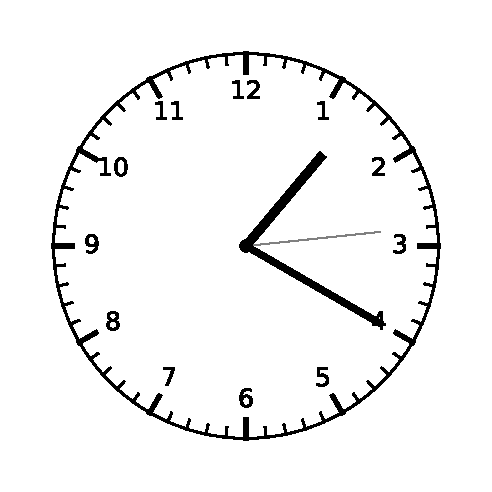
\includegraphics[width=0.5\textwidth]{maths/fig/clock_0120.pdf}} 
  What's the time? \dotfill\bigskip\par\dotfill\bigskip.
  
  \item Farmer Giles grew one thousand, nine hundred and ninety-eight singing potatoes.
  A flock of very hungry seagulls ate six hundred and eighty-nine of them.
  How many singing potatoes are left?\bigskip\par
Number sentence: \dotfill\bigskip\par
Answer: There are
\dotfill\bigskip\par\mbox{}\dotfill\bigskip\par\mbox{}\dotfill\bigskip\par\dotfill\bigskip
 singing potatoes left.

  \item Note on the Venn diagram where each of the following things belong:
  parakeets, rockets, ostriches, sugar gliders.\par
  {\centering 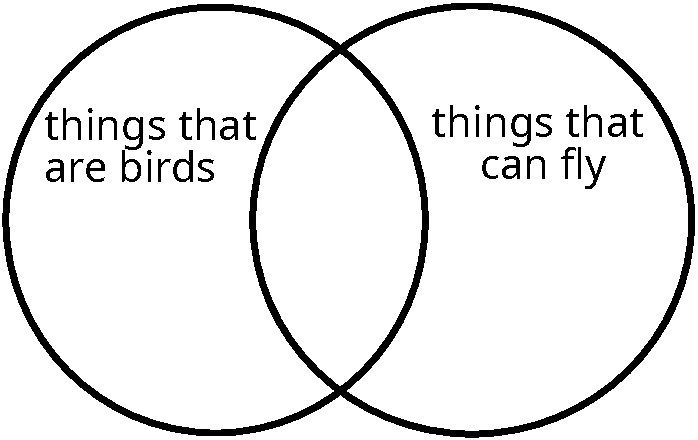
\includegraphics[width=0.8\textwidth]{maths/fig/venn_birds_fly.pdf}}

\end{enumerate}

\newpage\section{Problem Set \textnumero 2}

\begin{enumerate}
  \item Find ten nouns in this picture of a classroom.\bigskip
  \begin{marginfigure}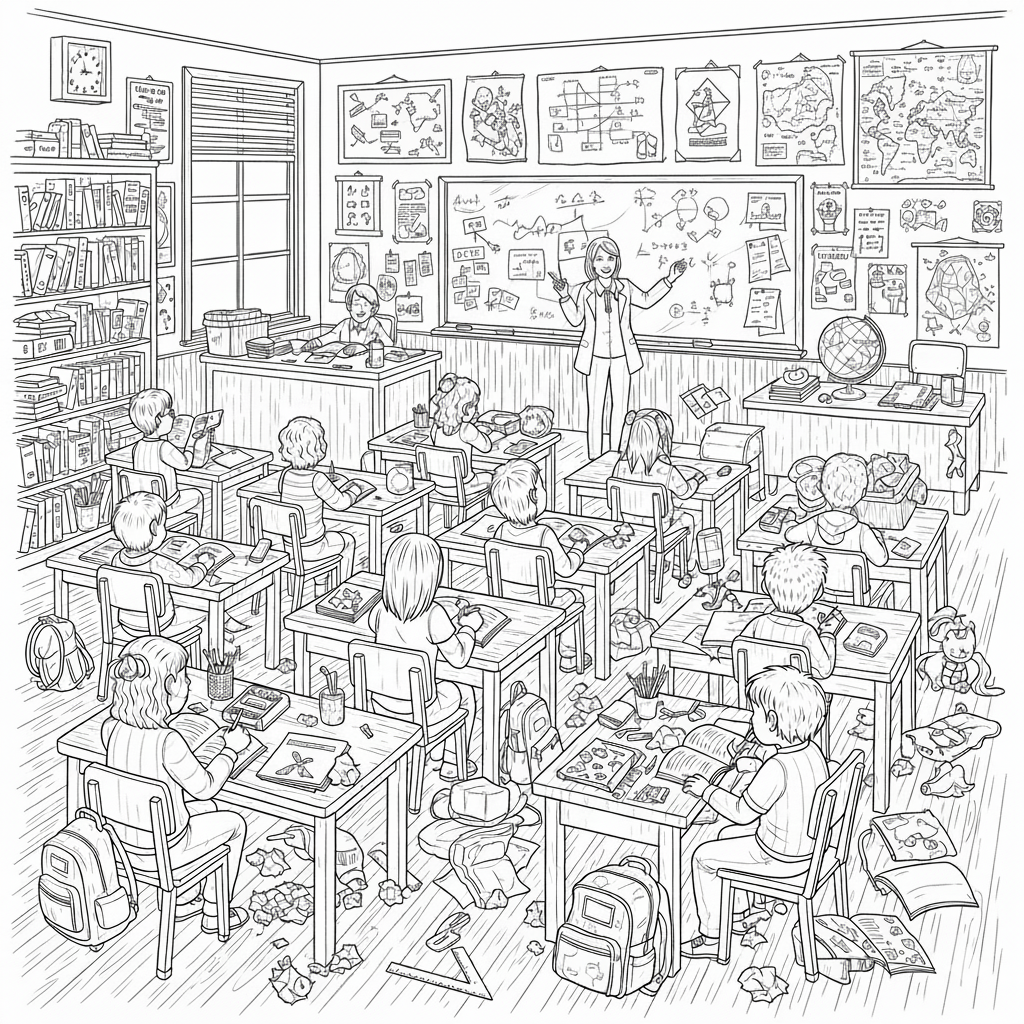
\includegraphics[width=\textwidth]{grammar/classroom.png}\end{marginfigure}
\begin{multicols}{2}
  \begin{enumerate}
    \item \dotfill\bigskip
    \item \dotfill\bigskip
    \item \dotfill\bigskip
    \item \dotfill\bigskip
    \item \dotfill
    \item \dotfill\bigskip
    \item \dotfill\bigskip
    \item \dotfill\bigskip
    \item \dotfill\bigskip
    \item \dotfill\bigskip
  \end{enumerate}
\end{multicols}

\item A grumpy gargoyle found seven hundred and sixty-five shiny bottle caps.
He then found two hundred and thirty-six more.
How many bottle caps does the gargoyle have in total?\bigskip\par
Number sentence: \dotfill\bigskip\par
Answer: The gargoyle has 
\dotfill\medskip\par\mbox{}\dotfill\medskip\par\mbox{}\dotfill\bigskip
 bottle caps in total.

\item The time is \dotfill\bigskip\par\dotfill\bigskip.
\begin{marginfigure}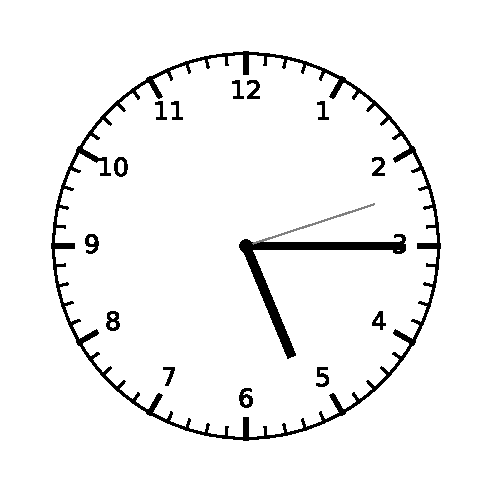
\includegraphics[width=\textwidth]{maths/fig/clock_0515.pdf}\end{marginfigure}

\item On the Venn diagram, note where each of the following things belong:
growl, speaking, snort, burp, giggle, meow.

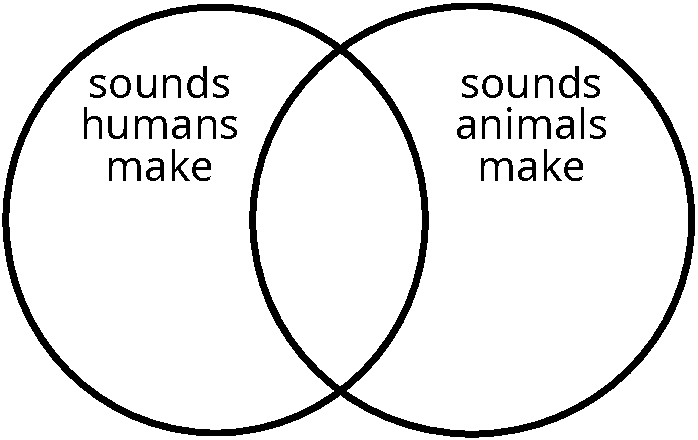
\includegraphics[width=0.9\textwidth]{maths/fig/venn_sounds.pdf}

\end{enumerate}

\clearpage\section{Problem Set \textnumero 3}

\begin{enumerate}
  \item Complete each sentence by filling in each blank with a \textbf{noun}.
  \begin{enumerate}
    \bigskip
    \item Princess Fluffybutt ate three\dotfill.\bigskip
    \item Professor Bumble wrote a \dotfill.\bigskip
    \item The \dotfill was chasing the \dotfill.\bigskip
    \item The sneaky cat broke the \dotfill.\bigskip
    \item The treasure chest contained \dotfill.\bigskip
  \end{enumerate}

  \item Princess Penelope likes animals. 
  She has eight unicorns, six penguins, twelve cats, a guinea pig, three puppies,
  one hundred and three mice, and a sugar glider.
  How many pets does Princess Penelope have in total?\bigskip\par
  Number sentence: \dotfill\bigskip\par
  Answer: Princess Penelope has \dotfill\bigskip\par\dotfill\bigskip pets.

  \item The time is \dotfill\bigskip\par\dotfill\bigskip.
  \begin{marginfigure}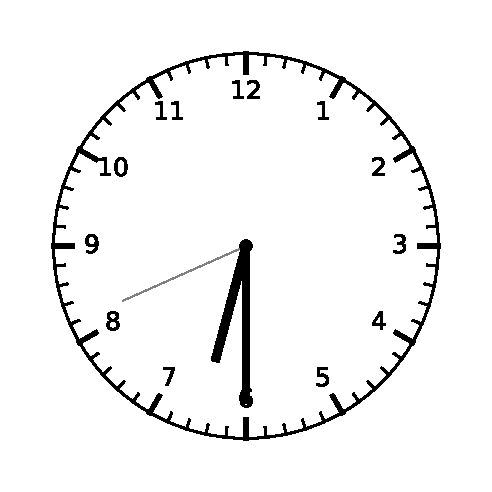
\includegraphics[width=\textwidth]{maths/fig/clock_0630.pdf}\end{marginfigure}

  \item The Venn diagram shows the elements of two sets, $A$ and $B$.
  \begin{marginfigure}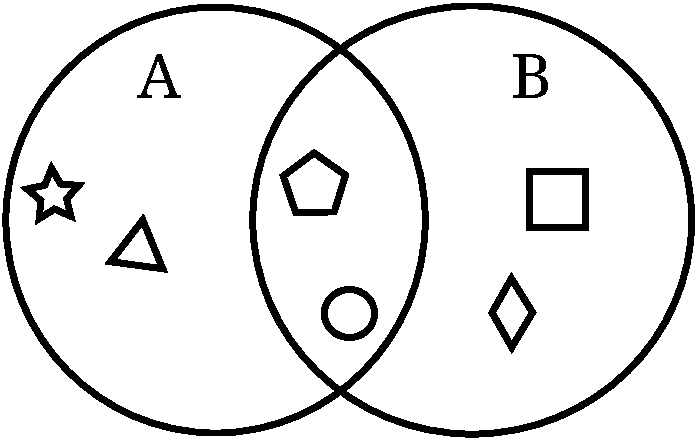
\includegraphics[width=\textwidth]{maths/fig/venn_sets.pdf}\end{marginfigure}
  What are the elements:
  \begin{enumerate}
    \item in set $A$:\dotfill\bigskip
    \item in set $B$:\dotfill\bigskip
    \item \emph{both} in set $A$ and in set $B$:\dotfill\bigskip
    \item in set {A} \emph{but not} in set {B}:\dotfill\bigskip
  \end{enumerate}

\end{enumerate}

\clearpage\section{Problem Set \textnumero 4}

\begin{enumerate}
  \item \marginnote{A \textbf{proper noun} starts with a capital letter and names a particular person, place, season, etc. Other nouns are called \textbf{common nouns}.}
  \underline{Underline} the proper nouns and \uwave{squiggle} under the common nouns in these sentences.
  \begin{enumerate}
    \item \underline{Spot} likes to chase \uwave{mice} in the \uwave{garden} during \underline{Spring}.
    \item Miss Fluffybutt is the principal of Fluffybutt Primary School.
    \item The garden is full of flowers in Summer.
    \item My school is located on Stinky Lane.
    \item Several students are having a picnic in the park.
    \item The old teacher is wearing a blue shirt.
    \item The students are having a picnic in the park.
  \end{enumerate}

  \item Princess Penelope had nine thousand, eight hundred and seventy-six soft toys.
  She gave eight thousand, nine hundred and eighty-eight of them away to charity. 
  How many soft toys does Princess Penelope have left?\bigskip\par
  Number sentence: \dotfill\bigskip\par
  Answer: Princess Penelope has \dotfill\bigskip\par\dotfill\bigskip soft toys left.

  \item The time is \dotfill\bigskip\par\dotfill\bigskip.
  \begin{marginfigure}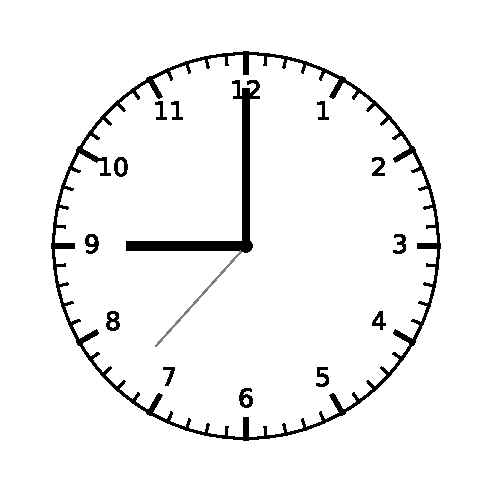
\includegraphics[width=\textwidth]{maths/fig/clock_0900.pdf}\end{marginfigure}

  \item Three boys go to school using a different methods at different speeds.
  The boy who rides his bike goes super fast. Ken does not walk.
  Russ travels at a medium pace. The person who travels slowly is walking.\par
  \begin{tabular}{|l|>{\centering}p{2cm}|>{\centering}p{2cm}|>{\centering}p{2cm}|>{\centering}p{2cm}|>{\centering}p{2cm}|>{\centering}p{2cm}|}
  \hline 
    & \textbf{Walking} & \textbf{Bike} & \textbf{Scooter} & \textbf{Super Fast} & \textbf{Medium} & \textbf{Slowly}\tabularnewline
  \hline 
  \textbf{Bob} &  &  &  &  &  & \tabularnewline
  \hline 
  \textbf{Ken} &  &  &  &  &  & \tabularnewline
  \hline 
  \textbf{Russ} &  &  &  &  &  & \tabularnewline
  \hline 
  \end{tabular}
  \bigskip
  \begin{itemize}
    \item Bob \dotfill\bigskip
    \item Ken \dotfill\bigskip
    \item Russ \dotfill
  \end{itemize}

\end{enumerate}

\clearpage\section{Problem Set \textnumero 5}

\begin{enumerate}
  \item \marginnote{\textbf{Countable nouns} can be counted (e.g. one apple, two apples).
  \textbf{Uncountable nouns} cannot be counted (e.g. sand, rain, sugar). Countable nouns usually form the plural by appending --s, but uncountable nouns do not.}
  Next to each noun, write "C" if it is countable, "U" if it is uncountable, or "CU" if it is both.
  \begin{multicols}{3}
  \begin{enumerate}
    \item apple: \dotfill
    \item car: \dotfill
    \item house: \dotfill
    \item wood: \dotfill
    \item water: \dotfill
    \item wine: \dotfill
    \item cheese: \dotfill
    \item pumpkin: \dotfill
    \item bread: \dotfill
    \item milk: \dotfill
    \item sugar: \dotfill
    \item salt: \dotfill
    \item pepper: \dotfill
  \end{enumerate}
  \end{multicols}

  \item The time is \dotfill\bigskip\par\dotfill\bigskip.
  \begin{marginfigure}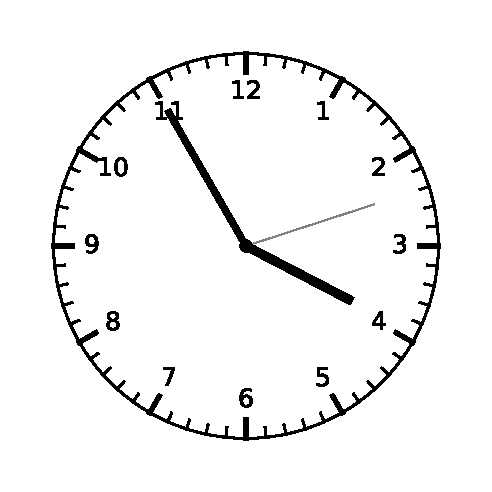
\includegraphics[width=\textwidth]{maths/fig/clock_0355.pdf}\end{marginfigure}

  \item \underline{Underline} the proper nouns and \uwave{squiggle} under the common nouns in these sentences.
  \begin{enumerate}
    \item Ben visited Paris with his family.
    \item Ben loves chocolate.
    \item The family ate too much chocolate and had to go for a walk.
    \item Ben and his sister felt very sick and had to go to the doctor.
    \item The doctor gave them some medicine to make them feel better.
    \item Ben's sister threw up all the chocolate she ate.
  \end{enumerate}

  \item Refer to the Venn diagram, then fill in the blanks with $\in$ or $\notin$.
  \begin{marginfigure}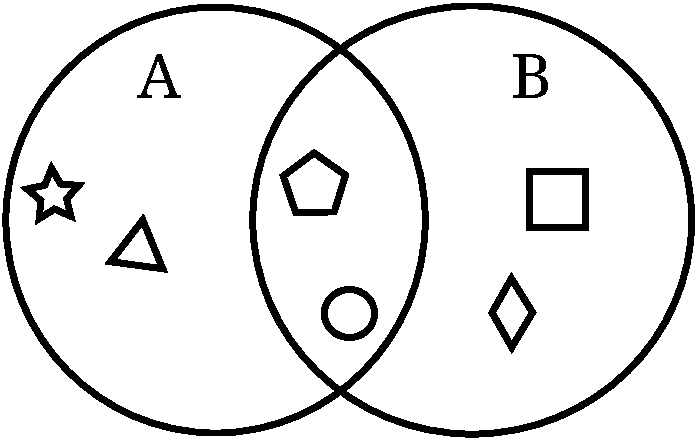
\includegraphics[width=\textwidth]{maths/fig/venn_sets.pdf}\end{marginfigure}
  \marginnote{If $\square$ is in set $S$, mathematicians write $\square \in S$. If $\square$ is not in set $S$, we write $\square \notin S$.}
  \begin{multicols}{4}
  \begin{enumerate}
    \item $\square$ \dotfill $A$\bigskip
    \item $\square$ \dotfill $B$\bigskip
    \item $\bigcirc$ \dotfill $A$\bigskip
    \item $\bigcirc$ \dotfill $B$\bigskip
    \item $\triangle$ \dotfill $A$\bigskip
    \item $\triangle$ \dotfill $B$\bigskip
  \end{enumerate}
  \end{multicols}
\end{enumerate}

\clearpage\section{Problem Set \textnumero 6}
\begin{enumerate}
  \item \begin{marginfigure}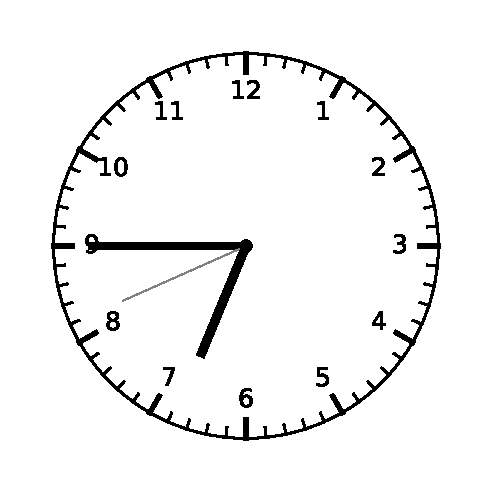
\includegraphics[width=\textwidth]{maths/fig/clock_0645.pdf}\end{marginfigure}
  The time is \dotfill\bigskip\par\dotfill\bigskip.\par

  \item \begin{enumerate}
  \item What is a proper noun? What kind of letter does it start with?\bigskip\par
  \dotfill\bigskip \par
  \dotfill
  
  \item Write down four proper nouns.
  \begin{multicols}{2}
  \begin{itemize}
    \item \dotfill\bigskip
    \item \dotfill\bigskip
    \item \dotfill\bigskip
    \item \dotfill\bigskip
  \end{itemize}
  \end{multicols}

  \item Now write down four common nouns.
  \begin{multicols}{2}
  \begin{itemize}
    \item \dotfill\bigskip
    \item \dotfill\bigskip
    \item \dotfill\bigskip
    \item \dotfill\bigskip
  \end{itemize}
  \end{multicols}
  \end{enumerate}

  \item Form the plurals of the following nouns:
  \marginnote{The plural form of a noun refers to more than one of that thing (one \emph{cat}, two \emph{cats}).}
  \marginnote{Most nouns form the plural by adding --s, but some nouns have irregular plurals (e.g. goose $\rightarrow$ geese).}
  \begin{multicols}{2}
  \begin{enumerate}
    \item cat: \dotfill\bigskip
    \item dog: \dotfill\bigskip
    \item book: \dotfill\bigskip
    \item tree: \dotfill\bigskip
    \item potato: \dotfill\bigskip
    \item tomato: \dotfill\bigskip
    \item leaf: \dotfill
    \item life: \dotfill\bigskip
    \item mouse: \dotfill\bigskip
    \item foot: \dotfill\bigskip
    \item child: \dotfill\bigskip
    \item person: \dotfill\bigskip
    \item woman: \dotfill\bigskip
    \item man: \dotfill\bigskip
  \end{enumerate}
  \end{multicols}
  
  \item 
  \marginnote{We describe the contents of sets using curly braces. For example, $S = \{1, 2, 3, 4, 5\}$ means that set $S$ contains the elements 1, 2, 3, 4, and 5.}
  Draw a Venn diagram to illustrate the sets
    $A = \{1, 2, 3, 4, 5\}$ and
    $B = \{2, 4, 6, 8\}$.
\end{enumerate}

\clearpage\section{Problem Set \textnumero 7}

\begin{enumerate}
  \item \begin{marginfigure}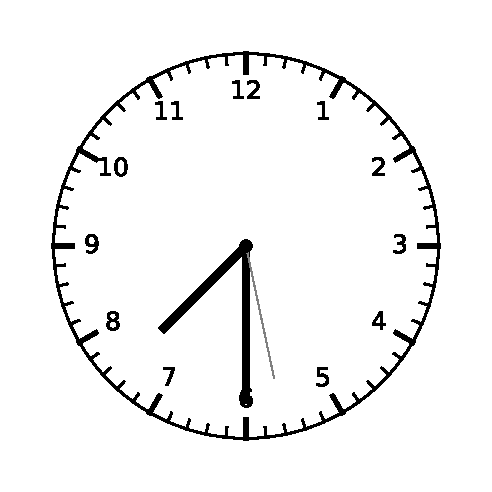
\includegraphics[width=\textwidth]{maths/fig/clock_0730.pdf}\end{marginfigure}
  The time is \dotfill\bigskip\par\dotfill\bigskip.\par

  \item Read the following passage, and find five common nouns and five proper nouns.
  \begin{quote}
    It shall be lawful for the Queen, with the advice of the Privy Council, to declare by proclamation that,
    on and after a day therein appointed, not being later than one year after the passing of this Act,
    the people of New South Wales, Victoria, South Australia, Queensland, and Tasmania, and also,
    if Her Majesty is satisfied that the people of Western Australia have agreed thereto, of Western Australia,
    shall be united in a Federal Commonwealth under the name of the Commonwealth of Australia.
    But the Queen may, at any time after the proclamation, appoint a Governor-General for the Commonwealth.
  \end{quote}
  \begin{itemize}
    \item[Five common nouns]: \dotfill\bigskip\par\dotfill\bigskip\par\dotfill\bigskip
    \item[Five proper nouns]: \dotfill\bigskip\par\dotfill\bigskip\par\dotfill\bigskip
  \end{itemize}

  \item   Barry the bee is a hard-working bee who counts the flowers he pollinates.
  How many did he pollinate the last three days? \bigskip\par
\marginnote{\begin{tabular}{|cc|}
  \hline 
  \textbf{Day} & \textbf{Flowers}\tabularnewline
  \hline 
  \textbf{Monday} & 142\tabularnewline
  \textbf{Tuesday} & 332\tabularnewline
  \textbf{Wednesday} & 96\tabularnewline
  \hline 
  \end{tabular}  
  }
  Number sentence: \dotfill\bigskip\par
  Answer: Barry pollinated \dotfill\bigskip\par\dotfill\bigskip flowers.

  \item Draw a Venn diagram for the sets
  $A = \{1, 2, 3, 4, 5\}$,
  $B = \{2, 4, 6, 8\}$, and
  $C = \{1, 2, 3, 15\}$.
  
\end{enumerate}

\clearpage\section{Problem Set \textnumero 8}

\begin{enumerate}
  \item What's the time on these clocks?\par
  \begin{fullwidth}
  \begin{tabular}{ccccc}
    (a) & (b) & (c) & (d) & (e) \\
    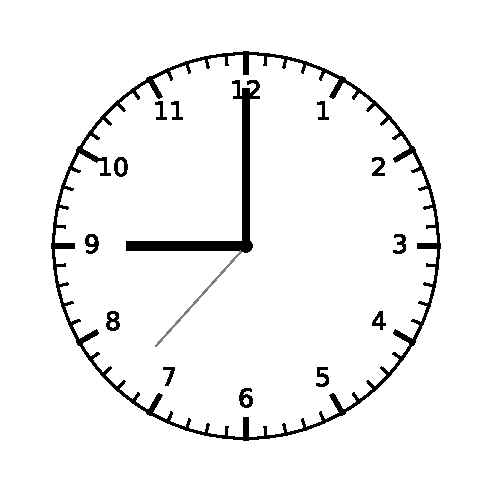
\includegraphics[width=0.25\textwidth]{maths/fig/clock_0900.pdf} &
    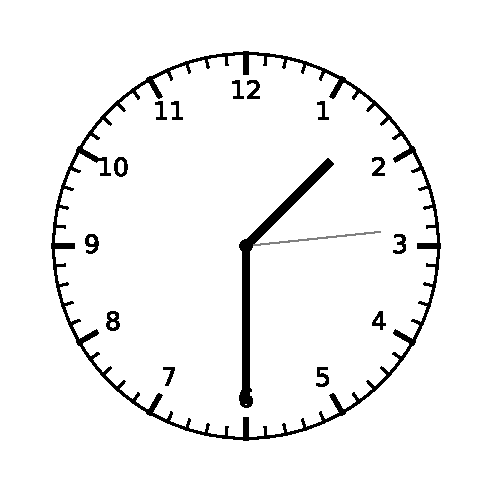
\includegraphics[width=0.25\textwidth]{maths/fig/clock_0130.pdf} &
    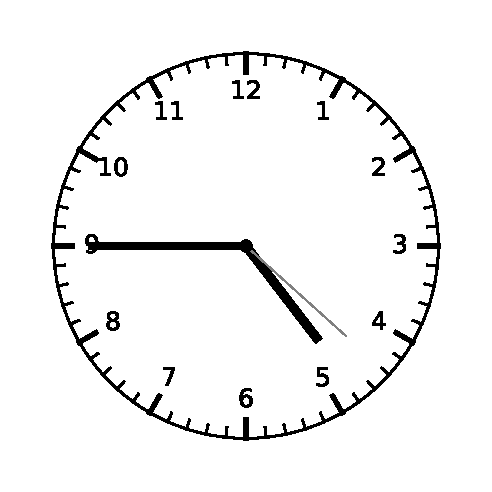
\includegraphics[width=0.25\textwidth]{maths/fig/clock_0445.pdf} &
    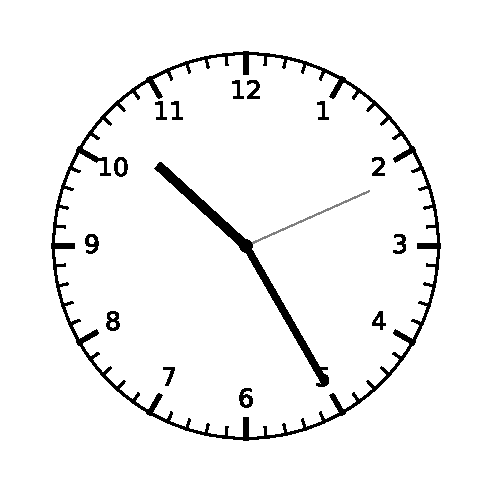
\includegraphics[width=0.25\textwidth]{maths/fig/clock_1025.pdf} &
    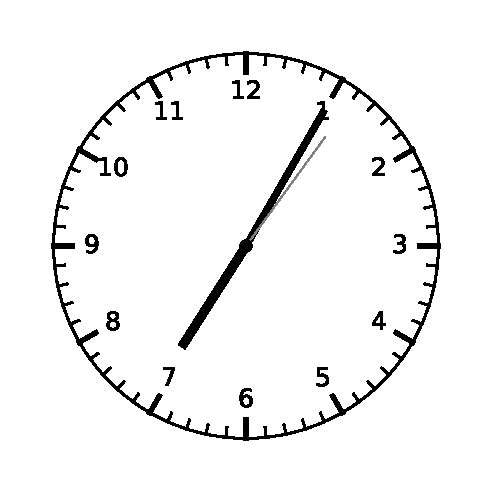
\includegraphics[width=0.25\textwidth]{maths/fig/clock_0705.pdf}
  \end{tabular}
  \bigskip
  \begin{enumerate}
    \item \dotfill\bigskip
    \item \dotfill\bigskip
    \item \dotfill\bigskip
    \item \dotfill\bigskip
    \item \dotfill
  \end{enumerate}
  \end{fullwidth}\bigskip

  \item Calculate: 1423 - 442 = \dotfill.

  \item Find four singular nouns and four plural nouns in the passage:
  \begin{quote}
    Sir Reginald Pigglesworth, a pig in a top hat, liked to collect rubber chickens. He had chickens of all sizes: a gigantic chicken that clucked like a tuba, three grumpy chickens who wore tiny spectacles, and a flock of baby chickens that squeaked like a thousand mice. Every evening, he would line up his prized possessions on the mantelpiece, polishing each one with a special cloth.
  \end{quote}
  \begin{enumerate}\bigskip
    \item Four singular nouns: \dotfill\bigskip\par\dotfill\bigskip\par\dotfill\bigskip
    \item Four plural nouns: \dotfill\bigskip\par\dotfill\bigskip\par\dotfill
  \end{enumerate}

  \item \begin{marginfigure}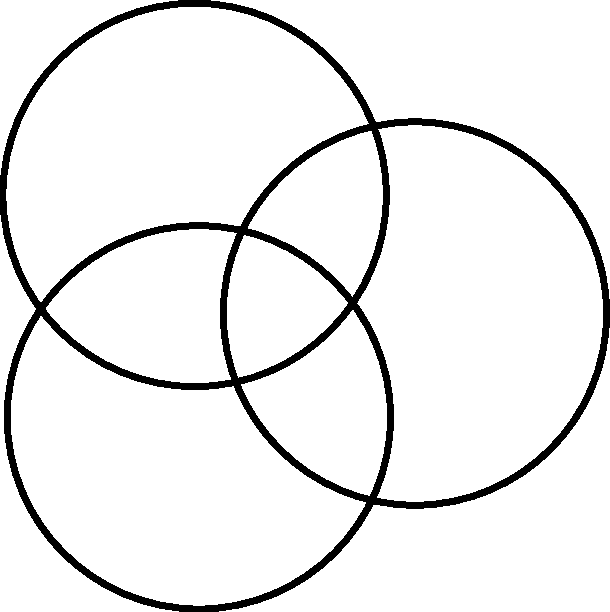
\includegraphics[width=\textwidth]{maths/fig/venn_blank_3.pdf}\end{marginfigure}
  Let $X := \left\{\clubsuit, \diamondsuit, \bigcirc, \times\right\}$, $Y := \left\{\diamondsuit, \heartsuit, \bigstar, \square\right\}$, and $Z := \left\{\diamondsuit, \bigstar, \triangle\right\}$. Complete the Venn diagram.
\end{enumerate}

\clearpage\section{Problem Set \textnumero 9}

\begin{enumerate}
  \item \underline{Underline} the verbs in these sentences.
  \marginnote{A \emph{verb} is a word that describes an action or a state of being (e.g. \emph{ran}, \emph{ate}).}
  \begin{enumerate}
    \item The cat sat on the mat.
    \item The dog chased the cat.
    \item The cat swiped at the dog.
    \item The dog ran away.
    \item The cat purred.
  \end{enumerate}

  \item Use a \emph{verb} to complete these sentences:\bigskip
  \begin{enumerate}
    \item I like to \dotfill\bigskip ice cream.
    \item Boris \dotfill\bigskip the ball.
    \item Andrew \dotfill\bigskip the plate on the floor.
    \item Emma \dotfill\bigskip the book.
  \end{enumerate}

  \item Let $X := \left\{\clubsuit, \diamondsuit, \bigcirc, \times\right\}$, $Y := \left\{\diamondsuit, \heartsuit, \bigstar, \square\right\}$, and $Z := \left\{\diamondsuit, \bigstar, \triangle\right\}$. \marginnote{The symbol $:=$ means `is defined as'.}
  Write `true' or `false' for each of the following statements:
  \marginnote{Remember, $\in$ means `is an element of' and $\notin$ means `is not an element of'.}
  \begin{multicols}{2}
  \begin{enumerate}
    \item $\clubsuit \in X$ \dotfill\bigskip
    \item $\diamondsuit \in Y$ \dotfill\bigskip
    \item $\bigstar \in Y$ \dotfill\bigskip
    \item $\square \notin Y$ \dotfill
    \item $\alpha \notin Z$ \dotfill\bigskip
    \item $\bigcirc \in X$ or $\bigcirc \in Z$ \dotfill\bigskip
    \item $\bigcirc \in Y$ or $\bigcirc \in Z$ \dotfill\bigskip
    \item $\times \in X$ and $\times \in Y$ \dotfill
  \end{enumerate}
  \end{multicols}

  \item I have a box of piffles. Some piffles are ongles and the rest are gingles.
  All of the ongles are red. Most of the gingles are blue. If I take a red piffle from the box,
  is it definitely an ongle? Explain your answer.\bigskip\par
  \dotfill\bigskip\par\dotfill\bigskip\par\dotfill.

\end{enumerate}

\clearpage\section{Problem Set \textnumero 10}

\begin{enumerate}
  \item \underline{Underline} the verbs:
  \marginnote{Remember, a \emph{verb} is a word that describes an action or a state of being (e.g., \emph{is}, \emph{ran}, \emph{ate}).}
  \begin{quote}
    We hold these truths to be self-evident, that all men are created equal, that they are endowed by their Creator with certain unalienable Rights, that among these are Life, Liberty and the pursuit of Happiness.
  \end{quote}
  \marginnote{This passage is from the American Declaration of Independence, written 250 years ago. Do you notice any differences in capitalisation rules, compared to modern English?}

  \item All of the boys in Mrs. Tutte's class have red hair.
  Some of the girls in the class have brown hair.
  Can Mrs. Tutte have a boy with brown hair in her class? Answer `yes' or `no' and give reasons.\bigskip\par
  \dotfill\bigskip\par\dotfill\bigskip\par\dotfill.

  \item Let $x$ represent some number. Suppose that $8 - x = 3.$
  What's $x$?\bigskip\par
  Number sentence: $x =$ \dotfill\bigskip\par
  Answer: $x$ is \dotfill.

  \item Refer to the Venn diagram, then write `true' or `false' for each of the following statements:
  \begin{marginfigure}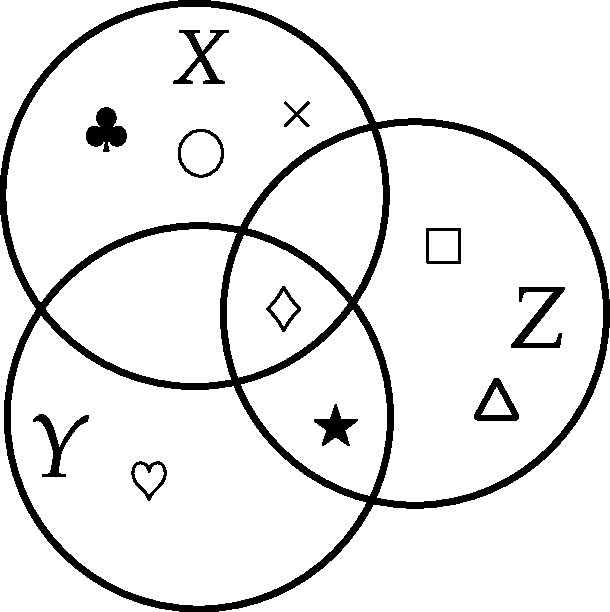
\includegraphics[width=\textwidth]{maths/fig/venn_3.pdf}\end{marginfigure}
  \begin{multicols}{2}
    \begin{enumerate}
      \item $\clubsuit \in X$ \dotfill\bigskip
      \item $\diamondsuit \in Y$ \dotfill\bigskip
      \item $\bigstar \in Y$ \dotfill\bigskip
      \item $\square \notin Y$ \dotfill
      \item $\bigstar \notin Z$ \dotfill\bigskip
      \item $\heartsuit \in X$ or $\heartsuit \in Z$ \dotfill\bigskip
      \item $\heartsuit \in Y$ or $\heartsuit \in Z$ \dotfill\bigskip
      \item $\diamondsuit \in X$ and $\diamondsuit \in Y$ \dotfill
    \end{enumerate}
    \end{multicols}

  \item Andrew bought 423 piffles. He sold 262 to Ben, who then sold six to Charlie.
  If everyone started out with no piffles, 
  how many piffles does Andrew now have?\bigskip\par
  Number sentence: \dotfill\bigskip\par
  Answer: Andrew now has \dotfill\bigskip\par\dotfill\bigskip\par\dotfill\bigskip piffles.
  
\end{enumerate}

\clearpage\section{Problem Set \textnumero 11}

\begin{enumerate}
  \item For each sentence, \underline{underline} the verb and \uwave{squiggle} under the nouns.
  \begin{enumerate}
    \item A whirlwind swept through the school.
    \item The wind lifted up the classroom's roof.
    \item The students ran to the bus stop.
    \item The teacher cancelled school for the day.
    \item The kids enjoyed their earlymark.
  \end{enumerate}

  \item I have two bags of ergles. Most of the ergles are blongies, some are jongies, and the rest are plongies.
  All of the blongies are red. Most of the jongies are blue and some are black.
  Some of the plongies are green but the rest are yellow.
  I pluck a blongie at random. What colour ergle did I choose?\bigskip\par
  \dotfill\bigskip\par\dotfill\bigskip\par\dotfill.

  \item Suppose that $\square + 4 = 12.$ What's the value of $\square$?\bigskip\par
  Number sentence: $\square =$ \dotfill\bigskip\par
  Answer: $\square$ is \dotfill.

  \item Refer to the Venn diagram.
  \begin{marginfigure}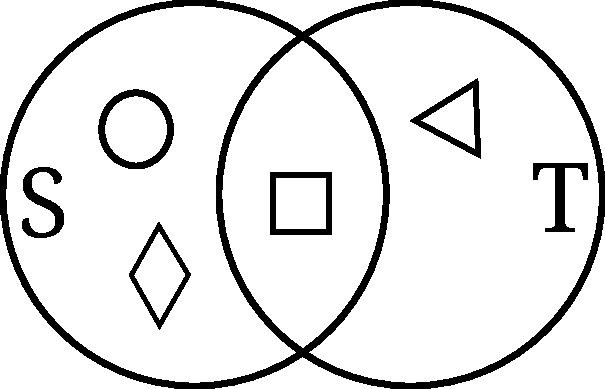
\includegraphics[width=\textwidth]{maths/fig/venn_2.pdf}\end{marginfigure}
  \marginnote{The \emph{intersection} of two sets is the set of elements that are in both sets.
  We write $S \cap T$ to mean the intersection of sets $S$ and $T$.}
  \marginnote{The \emph{union} of two sets is the set of elements that are in either set.
  We write $S \cup T$ to mean the union of sets $S$ and $T$.}
  \begin{enumerate}
    \item $S = \large\{$\dotfill$\large\}$\bigskip
    \item $T = \large\{$\dotfill$\large\}$\bigskip
    \item $S \cap T = \large\{$\dotfill$\large\}$\bigskip
    \item $S \cup T = \large\{$\dotfill$\large\}$\bigskip
  \end{enumerate}
\end{enumerate}

\clearpage\section{Problem Set \textnumero 12}

\begin{enumerate}
  \item \underline{Underline} the verbs, and \uwave{squiggle} under the nouns:
  \begin{quote}
    Jerry stepped into the bath. The water was warm. He splashed around and had fun.
    Then, he got out and dried himself off. He dressed himself, brushed his teeth, and went to bed.
  \end{quote}

  \item Look at the picture. Write down six \emph{verbs}, corresponding to actions in the picture.
  \begin{marginfigure}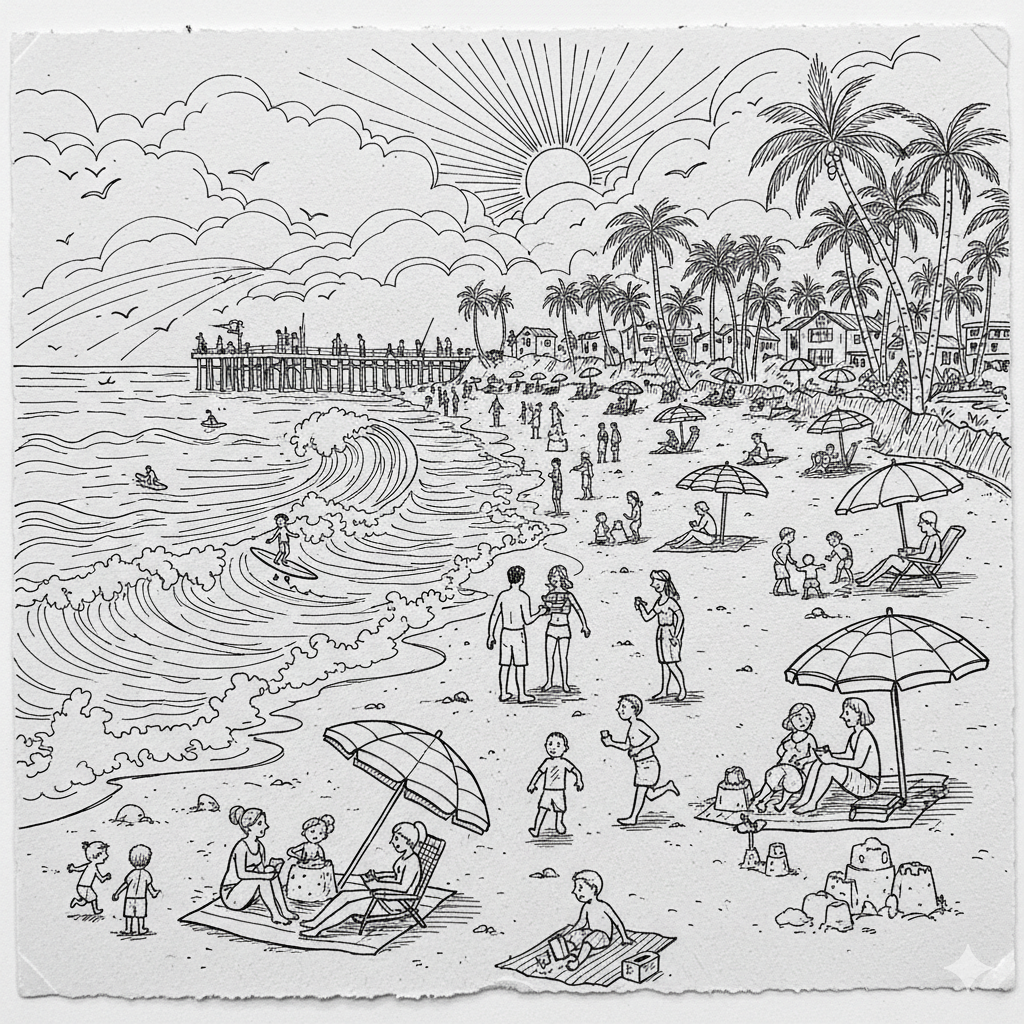
\includegraphics[width=\textwidth]{grammar/beach.png}\end{marginfigure}
  \begin{multicols}{2}
    \begin{enumerate}
      \item \dotfill\bigskip
      \item \dotfill\bigskip
      \item \dotfill
      \item \dotfill\bigskip
      \item \dotfill\bigskip
      \item \dotfill\bigskip
    \end{enumerate}
  \end{multicols}

  \item Let $X := \left\{1, 3, 5, 7\right\}$, and $Y := \left\{2, 3, 4, 5\right\}$.
  Write `true' or `false' for each of the following statements:
  \begin{multicols}{2}
    \begin{enumerate}
      \item $1 \in X$ \dotfill\bigskip
      \item $1 \in Y$ \dotfill\bigskip
      \item $1 \notin Y$ \dotfill\bigskip
      \item $3 \in X$ \dotfill
      \item $X \cap Y = \left\{3, 5\right\}$ \dotfill\bigskip
      \item $X \cup Y = \left\{1, 2, 3, 4, 5, 7\right\}$ \dotfill\bigskip
      \item $5 \in \left(X \cap Y\right)$ \dotfill\bigskip
      \item $5 \notin \left(X \cup Y\right)$ \dotfill\bigskip
    \end{enumerate}
  \end{multicols}
  
  \item Calculate: $2325 + 4196 =$ \dotfill.
\end{enumerate}

\clearpage\section{Problem Set \textnumero 13}

\begin{enumerate}
  \item \underline{Underline} the verbs, and \uwave{squiggle} under the nouns:
  \begin{quote}
    Licorice the cat woke up early. He stretched and went into the parents' bedroom.
    He jumped on the bed and woke Dad up. Dad got up and fed Licorice. Dad made coffee
    then let Licorice outside.
  \end{quote}

  \item Use a \emph{verb} to complete each sentence:
  \begin{multicols}{2}
  \begin{enumerate}
    \item Onk \dotfill a unicorn.\bigskip
    \item Rob \dotfill cake.\bigskip
    \item Mum \dotfill ice cream.
    \item I \dotfill a cat.\bigskip
    \item My dog \dotfill a shoe.\bigskip
    \item Bork \dotfill goo.
  \end{enumerate}
  \end{multicols}

  \item The chart shows how long the children played at the park each day in the last week.
  \begin{marginfigure}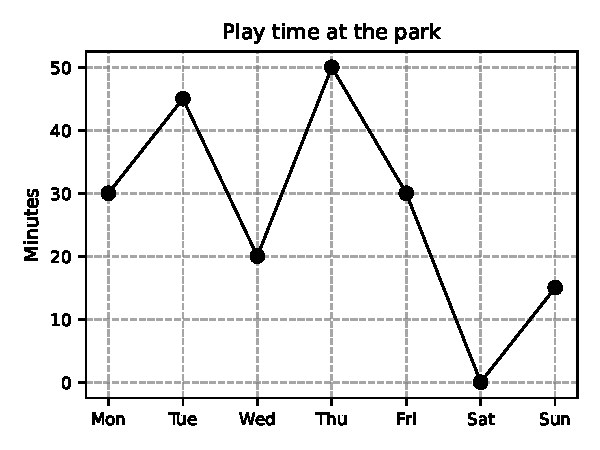
\includegraphics[width=\textwidth]{maths/fig/play_at_park.pdf}\end{marginfigure}
  \begin{enumerate}
    \item Did the kids play every day?\dotfill\bigskip
    \item When did they play the longest?\dotfill\bigskip
    \item How long did they play?\dotfill\bigskip
  \end{enumerate}

  \item Spronkus the unicorn found fifteen thousand, six hundred and thirty-two gold coins.
  He spent five thousand, two hundred and thirty-three of them on a golden castle. How many does he have left?\bigskip\par
  Number sentence: \dotfill\bigskip\par
  Answer: Spronkus has \dotfill\bigskip\par\dotfill\bigskip\par\dotfill\bigskip gold coins left.

  \item Define $X = \left\{a, b, c\right\}$, $Y = \left\{c, d, e\right\}$, and $Z = \left\{e\right\}$.
  \marginnote{Remember, $\cap$ means `intersection' (set overlap) and $\cup$ means `union' (everything together).}
  \begin{enumerate}
    \item $X \cap Y = $\dotfill\bigskip
    \item $X \cup Y = $\dotfill\bigskip
    \item $X \cap Z = $\dotfill\bigskip
    \item $X \cup Z = $\dotfill\bigskip
  \end{enumerate}
\end{enumerate}

\clearpage\section{Problem Set \textnumero 14}

\begin{enumerate}
  \item Complete each sentence with a \emph{verb}:
  \begin{multicols}{2}
  \begin{enumerate}
    \item Jim \dotfill bananas.\bigskip
    \item Toby \dotfill books.\bigskip
    \item I \dotfill pebbles.
    \item Em \dotfill a tiger.\bigskip
    \item We \dotfill a dog.\bigskip
    \item They \dotfill roses.
  \end{enumerate}
  \end{multicols}

  \item There are five million, two hundred and forty-three thousand, one hundred and twenty-three pixies
  in the Magic Forest. Two hundred and twenty-three thousand more arrive from Pixie Hollow.
  \begin{enumerate}\bigskip
    \item Use Arabic numerals to write the starting number of pixies:\dotfill\bigskip\par\dotfill\bigskip
    \item In Arabic numerals, how many arrived from Pixie Hollow?\dotfill\bigskip\par\dotfill\bigskip
    \item As a number sentence, how many pixies are there now?\dotfill\bigskip\par\dotfill\bigskip
    \item There are now \dotfill\bigskip\par
    \dotfill\bigskip\par\dotfill\bigskip\par\dotfill\bigskip pixies in the Magic Forest.
  \end{enumerate}
  
  \item Let $X = \left\{a, b, c\right\}$, $Y = \left\{c, d, e\right\}$, and $Z = \emptyset$. True or false?
  \marginnote{Remember, $\cap$ means `intersection', $\cup$ means `union', and $\emptyset$ is the empty set.}
  \begin{multicols}{2}
  \begin{enumerate}
    \item $X \cap Y = \left\{c\right\}$ \dotfill\bigskip
    \item $X \cup Y = \left\{a, b, c, d, e\right\}$ \dotfill\bigskip
    \item $X \cap Z = \emptyset$ \dotfill
    \item $X \cup Z = \left\{a, b, c\right\}$ \dotfill\bigskip
    \item $X \cap Z = Z$ \dotfill\bigskip
    \item $X \cup Y = Y$ \dotfill
  \end{enumerate}
  \end{multicols}

\end{enumerate}

\clearpage\section{Problem Set \textnumero 15}

\begin{enumerate}
  \item For each sentence, use the infinitive verb in parentheses to complete the sentence. You may use any tense you like.
  \marginnote{The \emph{infinitive} is the base form of the verb, without any tense or conjugation. It always starts with \textit{to}.
  For example, \textit{to eat} is the infinitive form of the verb in the sentence \textit{Harry eats bananas}.}
  \begin{enumerate}\bigskip
    \item (\textit{to eat}) Harry \dotfill bananas.\bigskip
    \item (\textit{to write}) Barry \dotfill books.\bigskip
    \item (\textit{to throw}) I \dotfill pebbles.\bigskip
    \item (\textit{to see}) Em \dotfill a tiger.\bigskip
    \item (\textit{to play}) We \dotfill with a dog.\bigskip
    \item (\textit{to smell}) They \dotfill roses.
  \end{enumerate}

  \item Complete each sentence with a \emph{noun}:
  \begin{enumerate}\bigskip
    \item Aaron eats \dotfill.\bigskip
    \item We have a \dotfill.\bigskip
    \item Rufus is chasing a \dotfill.\bigskip
    \item I saw a \dotfill.\bigskip
    \item They are flying a \dotfill.\bigskip
    \item Andrew is painting a \dotfill.\bigskip
  \end{enumerate}

  \item Define $X = \left\{1, 2, 3\right\}$, $Y = \left\{2, 3, 4\right\}$, and $Z = \left\{5\right\}$. True or false?
  \marginnote{Remember: $\cap$ means `intersection', $\cup$ means `union', and $\emptyset$ is the empty set.}
  \begin{multicols}{2}
  \begin{enumerate}
    \item $X \cap Y = \left\{2, 3\right\}$ \dotfill\bigskip
    \item $X \cup Y = \left\{1, 2, 3, 4\right\}$ \dotfill\bigskip
    \item $X \cup Z = \emptyset$\dotfill
    \item $X \cap Z = \emptyset$\dotfill\bigskip
    \item $3 \in \left(X \cap Y\right)$ \dotfill\bigskip
    \item $3 \notin \left(X \cup Y\right)$ \dotfill
  \end{enumerate}
  \end{multicols}
\end{enumerate}

\clearpage\section{Problem Set \textnumero 16}

\begin{enumerate}
  \item Complete each sentence with an \emph{article}.
  \marginnote{An \emph{article} introduces a noun. It can be \emph{indefinite} (\textit{a}, \textit{an}) or \emph{definite} (\textit{the}).}
  \begin{multicols}{2}
  \begin{enumerate}
    \item Kim broke \dotfill vase.\bigskip
    \item Tom had \dotfill book.\bigskip
    \item Bob ate \dotfill apple.\bigskip
    \item I saw \dotfill plane.
    \item They flew \dotfill plane.\bigskip
    \item Andrew painted \dotfill picture.\bigskip
    \item I made \dotfill mess.\bigskip
    \item They found \dotfill treasure.
  \end{enumerate}
  \end{multicols}

  \item Write the following numbers out in Arabic numerals:
  \marginnote{Remember the groupings:
  $$\underbrace{\text{\Large 123}}_\text{millions},\underbrace{\text{\Large 456}}_\text{thousands},\underbrace{\text{\Large 789}}_{\text{ones}}$$}
  \begin{enumerate}
    \item Four hundred and fifty-six\bigskip\par\dotfill\bigskip
    \item Twenty-three thousand, nine hundred and two\bigskip\par\dotfill\bigskip
    \item Eight million, seven hundred and sixty-five thousand, three hundred and twenty-one\bigskip\par\dotfill\bigskip
    \item Two hundred and eighty-seven million, six hundred and fifty-four thousand, three hundred and twenty-one\bigskip\par\dotfill\bigskip
    \item Nine hundred and ninety-nine million, nine hundred and ninety-nine thousand, nine hundred and ninety-nine\bigskip\par\dotfill\bigskip
  \end{enumerate}

  \item Calculate: $123,456 + 789,012 =$ \dotfill.
\end{enumerate}

\clearpage\section{Problem Set \textnumero 17}

\begin{enumerate}
  \item Construct sentences using the verb, nouns, and articles provided. Use any tense you like.
  \marginnote{Remember: sentences start with a capital letter and end with a full stop.}

  \begin{tabular}{|l|cccc|}
    \hline
    \textnumero & \textbf{Verb} & \textbf{First noun} & \textbf{Second noun} & \textbf{Article} \\
    \hline
    (a) & to eat & apple & Andrew & the \\
    (b) & to run & Em & race & the \\
    (c) & to see & Bob & tiger & a \\
    (d) & to play & Toby & flute & the \\
    (e) & to write & poem & Barry & a \\
    (f) & to draw & picture & Len & a \\
    \hline
  \end{tabular}
  \begin{enumerate}\bigskip
    \item \dotfill\bigskip
    \item \dotfill\bigskip
    \item \dotfill\bigskip
    \item \dotfill\bigskip
    \item \dotfill\bigskip
    \item \dotfill
  \end{enumerate}

  \item Define the sets
  $A = \{1, 2, 3\}$,
  $B = \{2, 4, 5\}$, and
  $C = \{3, 6\}$.
  \begin{marginfigure}
  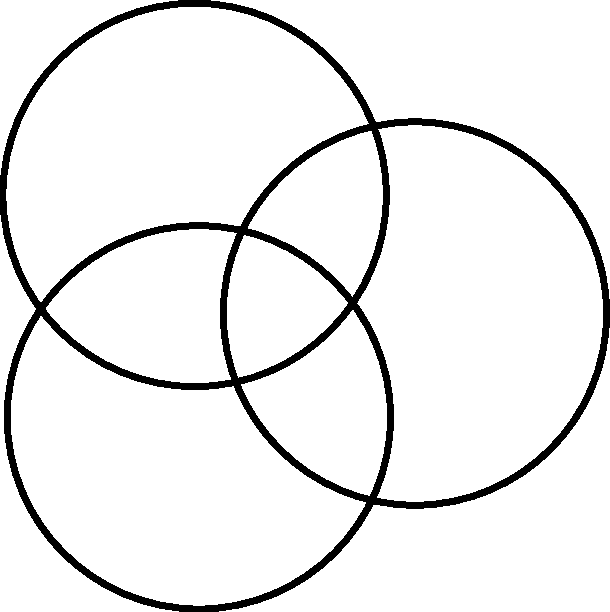
\includegraphics[width=\textwidth]{maths/fig/venn_blank_3.pdf}
  \end{marginfigure}
  \begin{enumerate}
    \item Complete the Venn diagram.\bigskip
    \item $A \cap B = \large\{$\dotfill$\large\}$\bigskip
    \item $B \cup C = \large\{$\dotfill$\large\}$
  \end{enumerate}

  \item Continue the arithmetic sequences:
  \begin{enumerate}\bigskip
    \item 105, 104, 103, \dotfill, \dotfill, \dotfill\bigskip
    \item 11, 13, 15, \dotfill, \dotfill, \dotfill\bigskip
    \item 85, 90, 95, \dotfill, \dotfill, \dotfill\bigskip
    \item 24, 22, 20, \dotfill, \dotfill, \dotfill
  \end{enumerate}
\end{enumerate}
\end{document}
